\documentclass[a4paper,11pt]{article}
\usepackage[T1]{fontenc}
\usepackage[utf8]{inputenc}
\usepackage{lmodern}
\usepackage{microtype}
\usepackage[top=2.5cm,bottom=2.5cm,left=2.5cm,right=2.5cm]{geometry}
\usepackage{booktabs}
\usepackage{graphicx}
\usepackage{xcolor}
\usepackage{array}
\usepackage[colorlinks=true,urlcolor=blue,linkcolor=blue]{hyperref}
\usepackage{fancyhdr}
\usepackage{caption}
\usepackage{amssymb}
\usepackage{pdflscape}

\definecolor{accent}{RGB}{52,152,219}

\pagestyle{fancy}\fancyhf{}
\lhead{\small\itshape Alan Crozier}
\rhead{\small\itshape Flavonoid research --- Author Report}
\rfoot{\small\thepage}
\renewcommand{\headrulewidth}{0.4pt}

\begin{document}

%% ── Title block ──────────────────────────────────────────────────────────────
\begin{center}
  {\LARGE\bfseries Alan Crozier}\\[0.4em]
  {\large\color{accent} Flavonoid research}\\[0.25em]
  {\normalsize University of Glasgow, GB}\\[0.15em]
  {\small\url{https://openalex.org/A5062888766}}
\end{center}
\vspace{0.4em}\noindent\rule{\linewidth}{0.5pt}\vspace{0.4em}


\section*{Profile}
\begin{quote}
\itshape
Here is a concise academic profile for Alan Crozier:

Alan Crozier is a prominent researcher in the field of flavonoid research at the University of Glasgow. With an impressive publication record of 60 papers, his work has garnered significant attention, with over 7,415 citations to date. This level of recognition is reflected in his network influence metrics, where he ranks among the top 0.5\% (PageRank percentile: 99.5\%) and is a key connector between different research communities (betweenness percentile: 98.1\%).

Crozier's research focuses on the chemistry, bioavailability, and health effects of dietary phenolics, with a particular emphasis on flavonoids and phenolic antioxidants in berries and other plant-based foods. His work has been published in leading journals and has contributed to our understanding of the absorption, metabolism, and excretion of these compounds. The breadth of his research is evident from the diverse range of topics covered in his papers, including the bioavailability and protective effects of berry flavonoids, the metabolome of polyphenolic compounds, and the colonic degradation and urinary excretion of flavan-3-ols.

Crozier's collaborative nature is also notable, with 143 co-authors across his publications. This level of interdisciplinary collaboration reflects his commitment to advancing our understanding of flavonoid research through a multidisciplinary approach.
\end{quote}
{\small\textcolor{gray}{Generated by a local language model via Ollama. Verify before use.}}
\bigskip

%% ── Metrics ──────────────────────────────────────────────────────────────────
\section*{Network Metrics and Field Ranks}

\begin{tabular}{p{6.5cm}rr}
\toprule
Metric & Value & Percentile\textsuperscript{$\dagger$} \\
\midrule
    Papers & 60 & 100.0\,\% \\
    Citations & 7415 & 100.0\,\% \\
    PageRank & 0.00392 & 99.5\,\% \\
    Betweenness centrality & 0.05456 & 98.1\,\% \\
    In-degree (cited by) & -- & --- \\
    Out-degree (cites others) & -- & --- \\
    Co-authors & 143 & --- \\
    First-author papers & 3 & --- \\
    Last-author papers & 33 & --- \\
\bottomrule
\end{tabular}

\smallskip
{\footnotesize $\dagger$\,Proportion of authors in the Flavonoid research corpus scoring below
this author. Betweenness is approximated for top-ranked authors only.}

%% ── Research breakdown ───────────────────────────────────────────────────────
\section*{Research Breakdown}

\noindent
\begin{minipage}[t]{0.46\linewidth}

\end{minipage}\hfill
\begin{minipage}[t]{0.46\linewidth}

\subsection*{Study types}
\begin{tabular}{lr}
\toprule
Study type & Papers \\
\midrule
    Other & 44 \\
    Review & 10 \\
    RCT & 5 \\
    Observational & 1 \\
\bottomrule
\end{tabular}

\end{minipage}


\section*{Sample Papers}
\begin{itemize}\setlength\itemsep{2pt}
  \item Dietary phenolics: chemistry, bioavailability and effects on health
  \item Identification of Flavonoid and Phenolic Antioxidants in Black Currants, Blueberries, Raspberries, Red Currants, and Cranberries
  \item Berry flavonoids and phenolics: bioavailability and evidence of protective effects
  \item The absorption, metabolism and excretion of flavan-3-ols and procyanidins following the ingestion of a grape seed extract by rats
  \item Evaluation of Phenolic Compounds in Commercial Fruit Juices and Fruit Drinks
  \item The metabolome of [2-14C](−)-epicatechin in humans: implications for the assessment of efficacy, safety and mechanisms of action of polyphenolic bioactives
  \item Green Tea Flavan-3-ols: Colonic Degradation and Urinary Excretion of Catabolites by Humans
  \item Phenyl-γ-valerolactones and phenylvaleric acids, the main colonic metabolites of flavan-3-ols: synthesis, analysis, bioavailability, and bioactivity
  \item Human studies on the absorption, distribution, metabolism, and excretion of tea polyphenols
  \item Absorption, metabolism and excretion of Choladi green tea flavan‐3‐ols by humans
  \item Absorption, metabolism, and excretion of green tea flavan‐3‐ols in humans with an ileostomy
  \item On-line high-performance liquid chromatography analysis of the antioxidant activity of phenolic compounds in green and black tea
  \item Berry (Poly)phenols and Cardiovascular Health
  \item Absorption, metabolism, distribution and excretion of (−)-epicatechin: A review of recent findings
  \item Phytochemical Profiles of Black, Red, Brown, and White Rice from the Camargue Region of France
\end{itemize}

%% ── Network figures ──────────────────────────────────────────────────────────
\begin{landscape}
\section*{Networks}

\noindent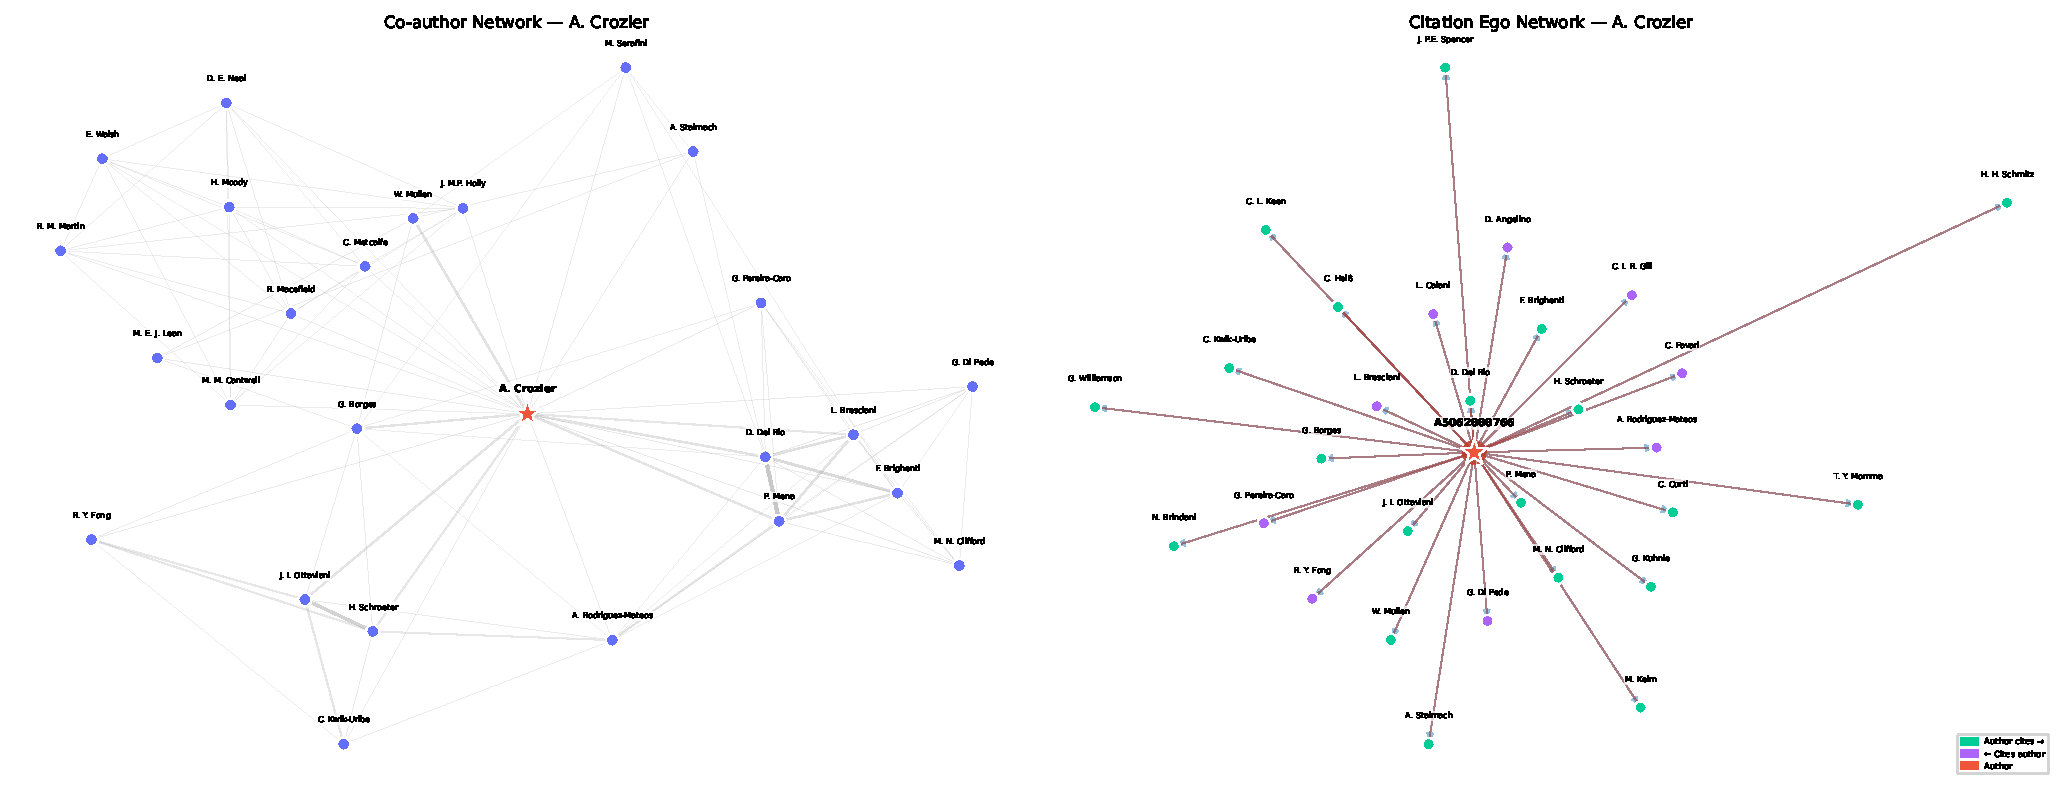
\includegraphics[width=\linewidth]{networks.pdf}

\noindent{\small
  \textbf{Left:} Co-author ego network. Edge width $\propto$ shared papers.
  \textbf{Right:} Citation ego network.
  \textcolor[RGB]{0,204,150}{Green} = authors this author cites;\;
  \textcolor[RGB]{171,99,250}{Purple} = authors who cite this author.\;
  $\bigstar$ = focal author.
}
\end{landscape}

\vfill
\noindent\rule{\linewidth}{0.4pt}\\
{\small Data source: \href{https://openalex.org}{OpenAlex}.
Metrics are computed within the Flavonoid research corpus and reflect
within-field standing only.
Generated \today.}

\end{document}
